\documentclass[10pt,a4paper,onecolumn]{article}
% \usepackage[utf8]{inputenc}
\usepackage{marginnote}
\usepackage{graphicx}
\usepackage{xcolor}
\usepackage{authblk,etoolbox}
\usepackage{titlesec}
\usepackage{calc}
\usepackage{hyperref}
\usepackage{bm}
\hypersetup{breaklinks=true,
            bookmarks=true,
            pdfauthor=
{
      Thierry D.G.A. Mondeel,
      Vivian Ogundipe,
      Hans V. Westerhoff,
  },
            pdftitle=
{
[Re] Predicting metabolic biomarkers of human inborn errors of metabolism
},
            colorlinks=true,
            citecolor=blue,
            urlcolor=blue,
            linkcolor=blue,
            pdfborder={0 0 0}}
\urlstyle{same}
\usepackage{tcolorbox}
\usepackage{ragged2e}
\usepackage{fontspec}
\usepackage{fontawesome}
\usepackage{caption}
\usepackage{listings}
\lstnewenvironment{code}{\lstset{language=Haskell,basicstyle=\small\ttfamily}}{}



%\usepackage{fancyvrb}
%\VerbatimFootnotes
%\usepackage{graphicx}
%\usepackage{mdframed}
%\newmdenv[backgroundcolor=lightgray]{Shaded}


\usepackage{longtable,booktabs}

\usepackage[
  backend=biber,
%  style=alphabetic,
%  citestyle=numeric
]{biblatex}
\bibliography{bibliography.bib}

\usepackage{amsmath,amssymb}



% --- Macros ------------------------------------------------------------------
\renewcommand*{\bibfont}{\small \sffamily}

\definecolor{red}{HTML}{CF232B}
\newcommand{\ReScience}{Re{\bfseries \textcolor{red}{Science}}}

\newtcolorbox{rebox}
   {colback=blue!5!white, colframe=blue!40!white,
     boxrule=0.5pt, arc=2pt, fonttitle=\sffamily\scshape\bfseries,
     left=6pt, right=20pt, top=6pt, bottom=6pt}

\newtcolorbox{repobox}
   {colback=red, colframe=red!75!black,
     boxrule=0.5pt, arc=2pt, left=6pt, right=6pt, top=3pt, bottom=3pt}

% fix for pandoc 1.14     
\newcommand{\tightlist}{%
  \setlength{\itemsep}{1pt}\setlength{\parskip}{0pt}\setlength{\parsep}{0pt}}

% --- Style -------------------------------------------------------------------
\renewcommand*{\bibfont}{\small \sffamily}
\renewcommand{\captionfont}{\small\sffamily}
\renewcommand{\captionlabelfont}{\bfseries}

\makeatletter
\renewcommand\@biblabel[1]{{\bf #1.}}
\makeatother

% --- Page layout -------------------------------------------------------------
\usepackage[top=3.5cm, bottom=3cm, right=1.5cm, left=1.5cm,
            headheight=2.2cm, reversemp, includemp, marginparwidth=4.5cm]{geometry}

% --- Section/SubSection/SubSubSection ----------------------------------------
\titleformat{\section}
  {\normalfont\sffamily\Large\bfseries}
  {}{0pt}{}
\titleformat{\subsection}
  {\normalfont\sffamily\large\bfseries}
  {}{0pt}{}
\titleformat{\subsubsection}
  {\normalfont\sffamily\bfseries}
  {}{0pt}{}
\titleformat*{\paragraph}
  {\sffamily\normalsize}


% --- Header / Footer ---------------------------------------------------------
\usepackage{fancyhdr}
\pagestyle{fancy}
%\renewcommand{\headrulewidth}{0.50pt}
\renewcommand{\headrulewidth}{0pt}
\fancyhead[L]{\hspace{-1cm}
\includegraphics[width=4.0cm]{rescience-logo.pdf}}
\fancyhead[C]{}
\fancyhead[R]{} 
\renewcommand{\footrulewidth}{0.25pt}

\fancyfoot[L]{\hypersetup{urlcolor=red}
              \sffamily \ReScience~$\vert$
              \href{http://rescience.github.io}{rescience.github.io}
              \hypersetup{urlcolor=blue}}
\fancyfoot[C]{\sffamily 1 - \thepage}
\fancyfoot[R]{\sffamily Sep 2015 $\vert$
                        Volume \textbf{1} $\vert$
                        Issue \textbf{1}}
\pagestyle{fancy}
\makeatletter
\let\ps@plain\ps@fancy
\fancyheadoffset[L]{4.5cm}
\fancyfootoffset[L]{4.5cm}

% --- Title / Authors ---------------------------------------------------------
% patch \maketitle so that it doesn't center
\patchcmd{\@maketitle}{center}{flushleft}{}{}
\patchcmd{\@maketitle}{center}{flushleft}{}{}
% patch \maketitle so that the font size for the title is normal
\patchcmd{\@maketitle}{\LARGE}{\LARGE\sffamily}{}{}
% patch the patch by authblk so that the author block is flush left
\def\maketitle{{%
  \renewenvironment{tabular}[2][]
    {\begin{flushleft}}
    {\end{flushleft}}
  \AB@maketitle}}
\makeatletter
\renewcommand\AB@affilsepx{ \protect\Affilfont}
%\renewcommand\AB@affilnote[1]{{\bfseries #1}\hspace{2pt}}
\renewcommand\AB@affilnote[1]{{\bfseries #1}\hspace{3pt}}
\makeatother
\renewcommand\Authfont{\sffamily\bfseries}
\renewcommand\Affilfont{\sffamily\small\mdseries}
\setlength{\affilsep}{1em}

\LetLtxMacro{\OldIncludegraphics}{\includegraphics}
\renewcommand{\includegraphics}[2][]{\OldIncludegraphics[width=12cm, #1]{#2}}


% --- Document ----------------------------------------------------------------
\title{[Re] Predicting metabolic biomarkers of human inborn errors of metabolism}

    \usepackage{authblk}
                        \author[1,*]{Thierry D.G.A. Mondeel}
                    \author[2]{Vivian Ogundipe}
                    \author[1, 3, 4]{Hans V. Westerhoff}
                            \affil[1]{Synthetic Systems Biology and Nuclear Organization, Swammerdam Institute
for Life Sciences, University of Amsterdam, The Netherlands}
                    \affil[2]{Department of Cell Biology, University Medical Center Groningen,
University of Groningen, The Netherlands}
                    \affil[3]{Molecular Cell Physiology, Amsterdam Institute for Molecules, Medicines
and Systems, VU University Amsterdam, The Netherlands}
                    \affil[4]{Manchester Centre for Integrative Systems Biology, School of Chemical
Engineering and Analytical Science, The University of Manchester, UK}
            
\date{\vspace{-5mm}
      \sffamily \small \href{mailto:d.g.a.mondeel@uva.nl (thierry.mondeel@gmail.com)}{d.g.a.mondeel@uva.nl (thierry.mondeel@gmail.com)}}


\setlength\LTleft{0pt}
\setlength\LTright{0pt}


\begin{document}
\maketitle

\marginpar{
  %\hrule
  \sffamily\small
  %\vspace{2mm}
  {\bfseries Editor}\\
  Name Surname\\

  {\bfseries Reviewers}\\
        Name Surname\\
        Name Surname\\
  
  {\bfseries Received}  Sep, 1, 2015\\
  {\bfseries Accepted}  Sep, 1, 2015\\
  {\bfseries Published} Sep, 1, 2015\\

  {\bfseries Licence}   \href{http://creativecommons.org/licenses/by/4.0/}{CC-BY}

  \begin{flushleft}
  {\bfseries Competing Interests:}\\
  The authors have declared that no competing interests exist.
  \end{flushleft}

  \hrule
  \vspace{3mm}

  \hypersetup{urlcolor=white}
  
    \vspace{-1mm}
  \begin{repobox}
    \bfseries\normalsize
      \href{http://github.com/rescience/rescience-submission/article}{\faGithubAlt~Article repository}
  \end{repobox}
      \vspace{-1mm}
  \begin{repobox}
    \bfseries\normalsize
      \href{http://github.com/rescience/rescience-submission/code}{\faGithubAlt~Code repository}
  \end{repobox}
        \hypersetup{urlcolor=blue}
}

\begin{rebox}
\sffamily {\bfseries A reference implementation of}
\small
\begin{flushleft}
\begin{itemize}
    \item[→] T. Shlomi, M.N. Cabili, E. Ruppin, Predicting metabolic biomarkers of
human inborn errors of metabolism, Mol. Syst. Biol. 5 (2009) 263.
doi:10.1038/msb.2009.22.
  \end{itemize}\par
\end{flushleft}
\end{rebox}


\section{Introduction}\label{introduction}

Shlomi et al. \autocite{Shlomi2009} have developed a way in which flux
variability analysis \autocite{Mahadevan2003} is used to predict
biomarkers for inborn errors of metabolism (IEMs). The approach focuses
on exchange reactions in a metabolic network that connect extracellular
metabolites that reside in a medium, which might correspond to the
blood, to a reservoir such as the urine. The method then determines the
ranges of exchange fluxes that are compatible with constraints set by
the network's topology, flux bounds of reactions and the requirement of
steady state for each metabolite. Shlomi et al. proposed that if any
such ranges shift convincingly when the network contains a mutation, the
concentration ranges of the corresponding metabolites in the reservoir
should shift in parallel and these metabolites would therefore be
biomarkers.

Shlomi et al. illustrated the method first on a virtual metabolic map
and further validated their technique using the reconstruction of the
human metabolic map Recon1 \autocite{Duarte2007} empirically with
respect to known biomarkers, but did not provide any formal proof. For a
set of 17 IEMs that affect amino acid metabolism, they found 56\% of the
biomarkers that are correctly predicted and 76\% of predicted biomarkers
that were predicted correctly in terms of whether they increased or
decreased in concentration. Thiele et al. \autocite{Thiele2013} later
found an even higher precision using essentially the same FVA
methodology on an updated version of the metabolic reconstruction.

Below, we first introduce the essential vocabulary and concepts
necessary for understanding the method proposed by Shlomi et al.

\subsection{Definitions}\label{definitions}

Exchange reactions are reactions in the metabolic network that allow
import and/or export of metabolites from the metabolic map. Exchange
reactions are represented by non-mass-balanced pseudoreactions, e.g.
\(X \leftrightarrow \varnothing\). Positive flux indicates net secretion
of \(X\) by the cell and negative flux indicates the net uptake of
\(X\).

We define boundary metabolites to be metabolites that are involved in
exchange reactions with the environment, i.e.~they serve as inputs
and/or outputs for the metabolic network, e.g.~glucose and CO\(_2\).
These metabolites typically exist both inside and outside the cell.

Each boundary metabolite will be associated with the range of flux its
exchange reaction supports under the following constraints for the flux
distributions in the model: (i) network topology, (ii) mass-balance for
all metabolites, (iii) flux bounds of reactions in the network.
Optionally, there is an additional constraint of being optimal with
respect to attaining or maximizing a certain set of fluxes, the
``objective'', in the model.

Biomarkers are those boundary metabolites the range of exchange flux of
which differs between the wild-type (WT) and mutant simulations. Shlomi
et al. proposed a threshold of at least 10\% difference in the lower or
upper bounds of the wild-type vs.~the mutant flux intervals.

Each biomarker will be associated with a prediction for being either
elevated or decreased in the mutant case, as compared to the wild type.
A biomarker is considered to have an increased, or reduced,
extracellular concentration in the mutant case if, when plotting the
wild-type and mutant flux-variability intervals on a horizontal axis,
both the lower and upper boundary of the mutant interval are shifted to
the right, or left, respectively (see Figures
~\ref{fig:Shlomi2009_figure_1}B and ~\ref{fig:Shlomi2009_figure_3}B). If
the two borders of the mutant interval move in opposite directions with
respect to the wild-type interval, the result is scored as `unchanged'
and the boundary metabolite is not considered to be a biomarker.

\subsection{Flux variability
calculations}\label{flux-variability-calculations}

Flux ranges for boundary metabolites, consistent with the requirements
of a steady state and constraints on reaction reversibilities, may be
calculated by applying flux variability analysis
\autocite{Mahadevan2003}. Mathematically, flux variability analysis for
a specific exchange reaction \(v_i\) entails the following linear
programming problem:

\begin{align}
\text{Min } v_i \text{ or Max } &v_i, \text{ such that for all } k \nonumber \\
\bm{S} \bm{v} &= \bm{0} \nonumber \\
Z  &\geq \phi Z_{\text{max}} \nonumber \\
\alpha_k \leq & ~ v_k \leq \beta_k 
\end{align}

Here \(\bm{v}\) is the column vector of fluxes representing all
reactions in the model, \(v_i\) is the flux of the exchange reaction of
a given boundary metabolite \(i\), \(\alpha_k\) is the, possibly
negative, lower bound for reaction \(k\) and similarly \(\beta_k\) is
the, possibly negative, upper bound for reaction \(k\). The reaction
bounds are the \(V_{max}\)'s of the reactions and are part of the
metabolic network definition, typically they are set to either \(0\) or
\(\pm 1000\) if the true, biological, \(V_{max}\)'s are not known. These
values allow specification of irreversible reactions by setting the
lower bound (or upper bound) to zero. The index \(i\) specifies a single
reaction that is to be maximized, whereas the index \(k\) is used to
index the bound constraints that exist for each reaction, including
\(v_i\). \(v_i\) may be maximized in the forward (positive flux) or the
reverse (negative flux) direction if allowed by the bounds on \(v_i\).
For a network with \(m\) metabolites and \(r\) reactions, i.e.~fluxes,
\(\bm{S}\) is the stoichiometry matrix for the network of size
\(m \times r\). The numeric, typically integer, elements of \(\bm{S}\)
represent the stoichiometry coefficients of each metabolite \(m\) in
each reaction \(r\). \(Z = \bm{c}^T \bm{v}\) is the objective function
defined for the map, entailing a linear combination, defined by column
vector \(\bm{c}\), of one or more reactions. The vector \(\bm{c}\) is an
indicator of objective reactions, i.e.~it contains a value of \(1\) in
rows corresponding to fluxes that are to be included in the objective,
and zeros in all other rows. Due to the vector multiplication
\(\bm{c}^T \bm{v}\), the objective \(Z\) sums the fluxes of the
reactions that correspond to rows containing a value of \(1\) in
\(\bm{c}\). \(Z_{\text{max}}\) denotes the maximal value of the
objective function. We define \(0 \leq \phi \leq 1\) to be an arbitrary
minimal fraction of the maximal objective function value that has to be
achieved. When \(\phi=1\) we ask for the range of flux allowed for
reaction \(v_i\) while maintaining the maximal value of the linear
combination of objective fluxes. When setting \(\phi = 0\), one is
asking for the allowable flux range through reaction \(v_i\) regardless
of the value of the objective function (although the sign has to be
maintained). The latter, i.e. \(\phi=0\), is the case considered in the
method by Shlomi et al. The choice of \(\phi\) matters because when
\(\phi \neq 0\) we are requiring flux to flow through the set of
objective reactions (unless \(Z_{\text{max}} = 0\)). This may entail a
forced directionality through reactions that are required to ultimately
produce flux in the objective reactions. These additional limitations in
the freedom of the flux pattern may subsequently impact the biomarker
predictions. The approach discussed here entails predictions purely
based on the network topology and therefore sets \(\phi = 0\).

\subsection{Reference implementation}\label{reference-implementation}

The source code for the original publication is not publicly available
and the computation environment used was not mentioned in the
publication. The \href{https://github.com/opencobra/cobratoolbox}{MATLAB
COBRA toolbox} contains code to reproduce the analysis by Thiele et al.
but this was also performed in MATLAB.

We here present an implementation of the biomarker prediction method
originally proposed by Shlomi et al., programmed in Python, and
reproduce the results presented in Figure 1A-B, 2 and 3 of the original
publication. These figures concern the method's application to a simple
metabolic map and then to a set of \(17\) amino acid metabolism
disorders. Our Python module provides the biomarker prediction algorithm
and is agnostic of the map used. It can therefore be applied to other
maps than the human metabolic reconstruction considered by Shlomi et al.
Jupyter notebooks are provided that generate the illustrative map and
reproduce all results referred to in Figures 1A-B, 2 and 3 of Shlomi et
al. Our implementation is based on information given in the original
paper. However, some details critical to the reproduction were left
unexplained there and are highlighted here. We also include a more
detailed discussion of one of the amino acid IEMs to examine the
robustness of the predictions made using this approach. We feel this
adds to the utility of this reference implementation and the
understanding of the approach introduced by Shlomi et al.

\section{Methods}\label{methods}

\subsection{Overview}\label{overview}

We implemented the method of Shlomi et al. in Python. Our Python
function has several input parameters, most of which are optional in
order to enable the user to perturb the network in various ways and to
try variations of the method that differ from the ones implemented here
or in Shlomi et al. The default settings are such that they mimic the
approach Shlomi et al. originally proposed. All flux-variability
analyses are performed using COBRApy \autocite{Ebrahim2013}.

All simulations discussed here were performed in Python 3.6 using
COBRApy \autocite{Ebrahim2013} (version 0.9) and Pandas (version
0.20.3). This repository also functions in conjunction with
\href{http://mybinder.org}{MyBinder} which allows for full
reproducibility in the `cloud' without any need for installation of
additional software.

The rest of this section introduces the approach proposed by Shlomi et
al. as we implemented it.

\subsection{Implementation of the
algorithm}\label{implementation-of-the-algorithm}

Here, we examine inborn errors of metabolism (IEMs) resulting from
loss-of-function mutations in a single enzyme \(r\) that may catalyse
multiple chemical reactions. For IEMs that disrupt the activity of
several reactions, Shlomi et al. proposed applying the approach to each
reaction individually and then combining the list of biomarkers.

Therefore, for a given IEM we loop the following sequence of steps for
each affected reaction \(r\) and for each boundary metabolite \(m\):

\begin{enumerate}
\def\labelenumi{\arabic{enumi}.}
\tightlist
\item
  Compute the exchange flux interval of \(m\), when \(r\) is forced to
  be active with a flux of at least \(\epsilon \geq 0\). By default
  \(\epsilon = 1\). We refer to this as the forward wild-type interval
  \(WT_{r,m}^+\).
\item
  For reversible reactions \(r\), if the forward interval yields a flux
  range of \([0,0]\), constrain the flux to be negative and lower than
  \(-\epsilon \leq 0\), and compute the backward wild-type interval
  \(WT_{r,m}^-\).
\item
  The wild-type interval \(WT_{r,m}\) is equal to the union of the
  forward and backward intervals.
\item
  Compute the exchange flux interval of \(m\) when \(r\) is forced to be
  inactive by temporarily setting the lower and upper bound of \(r\) to
  zero. This interval is denoted by \(M_{r,m}\).
\item
  Compare the wild-type and mutant intervals and predict whether the
  external concentration of \(m\) increases, decreases or remains
  unchanged when reaction \(r\) is forced to be inactive. This is done
  by the following rule: if both boundaries are higher in the mutant
  simulation than the corresponding boundaries in the wild-type
  simulation, then \(m\) is predicted to be a biomarker and elevated. If
  both boundaries are lower in the mutant simulation as compared to the
  wild-type simulation, then the metabolite is predicted to be a
  biomarker and reduced. If the predicted changes are smaller than 10\%,
  \(m\) is a low confidence biomarker. When the wild-type and mutant
  intervals are disjoint intervals, \(m\) is a highly confident (H.C)
  biomarker.
\end{enumerate}

After the loop (steps 1-5) is completed, contradictory predictions for
\(m\) between the affected reactions \(r\) are dealt with based on a
majority rule. When there is an equal number of elevated and reduced
predictions, the boundary metabolite is considered to be unchanged,
i.e.~not a biomarker.

The flux variability analyses that yield the exchange flux intervals
computed in step 1, 2 and 4 are handled by the
flux\_analysis.variability.flux\_variability\_analysis function in
Cobrapy. The input for this function comprises the model, along with its
associated flux bounds which change during step 1, 2 and 4, the list of
reactions for which to calculate the flux intervals and a fraction of
the optimal objective flux to minimally obtain (fraction\_of\_optimum).
In our case we pass the model with flux bounds as described above, lists
of exchange reactions for the metabolites of interest and a fraction of
optimum of zero.

\section{Results}\label{results}

In this section we start with an analysis of the sensitivity of the
method which was not clearly discussed in the original publication but
is easily facilitated with our reference implementation. Subsequently,
we discuss the reproduction of Figures 1, 2 and 3 from the original
publication.

\subsection{Robustness of the flux variability
method}\label{robustness-of-the-flux-variability-method}

Shlomi et al. did not discuss in detail the effects of changing various
parameter settings of, and assumptions inherent to, their FVA-based
method, nor did they present a proof of any generality. Because our
Python implementation allows the user to set various parameters, it
becomes possible to illustrate how specific settings in the approach
proposed by Shlomi et al. affect the outcome of the simulations. An
example of the potential pitfalls and issues with this method is
investigated below, in which we look at predictions for the inborn error
of metabolism known as Phenylketonuria (PKU). Here, we simulate this
disease by applying one of its potential causes, i.e.~dysfunctionality
of the enzyme converting phenylalanine into tyrosine.

PKU patients are known for elevated levels of phenylalanine and
decreased levels of tyrosine in their serum. We illustrate this briefly
in an example also considered in Figure 2 of Shlomi et al. In Figure
~\ref{fig:PKU_network}, we sketched some essential features of the
metabolic network surrounding the phenylalanine hydroxylase (PAH) enzyme
that malfunctions in PKU. Unless stated otherwise, the simulations are
performed with a medium that allows efflux through all exchange
reactions with an upper bound of \(1000\) and influx through all
exchange reactions with a lower bound of \(-1\) and we use the default
settings, including a 10\% significance threshold. The only considered
biomarkers are the \(20\) proteinogenic amino acids. We will consider
six cases in total. The results are summarized in Table
~\ref{tbl:PKU_results}.

\begin{figure}
\centering
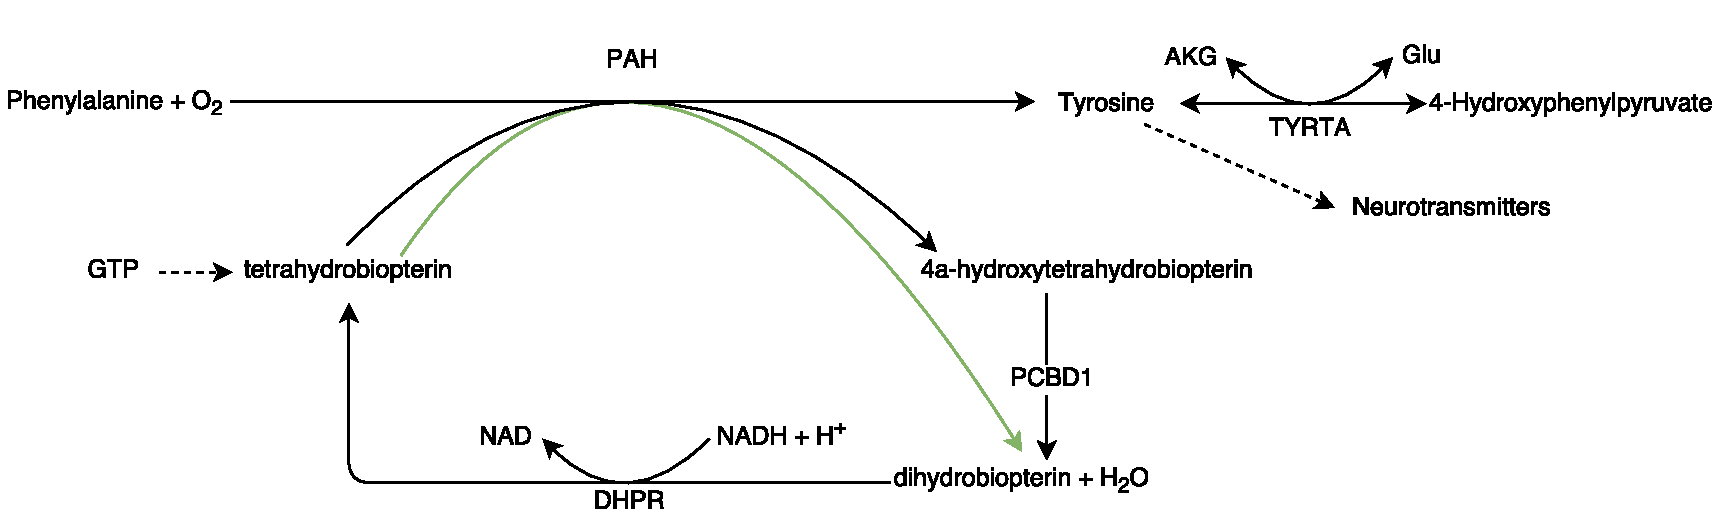
\includegraphics{./Figures/PKU_network.pdf}
\caption{Scheme of the network surrounding phenylalanine hydroxylase
(PAH) and its cofactors. The 4a-hydroxytetrahydrobiopterin produced by
PAH may spontaneously or when catalysed by PCBD1 (EC 4.2.1.96) dehydrate
to dihydrobiopterin which may be enzymatically reduced back by NADPH +
\(H^+\) to tetrahydrobiopterin through DHPR (EC 1.5.1.34). The solid
black lines indicate reactions that are contained in both Recon 1 and
Recon 2.2 \autocite{Swainston2016}. The solid green line refers to the
alternative PAH reaction that includes the spontaneous dehydradation
towards dihydrobiopterin that is only present in Recon 2.2. Dashed lines
indicate sources of the synthesis pathways or terminal products of the
indicated metabolites. The tyrosine transaminase (TYRTA) uses
oxoglutarate (AKG) and glutamate (Glu) as
cosubstrates.}\label{fig:PKU_network}
\end{figure}

Perhaps the most fundamental question is: can changes in network
topology result in different predictions? The answer is yes. One
illustration of this is the comparison of predictions between Recon 1
and Recon 2. As Table ~\ref{tbl:PKU_results} indicates, using the same
medium and algorithm settings for both Recon 1 and Recon 2.2, the two
networks led to different predictions of the effect of a defect of
phenylalanine hydroxylase on tyrosine. The application of the flux
variability method to Recon 1 correctly predicted both tyrosine and
phenylalanine as biomarkers as well as the directionality of the change
in their concentrations. In contrast, the prediction based on Recon 2.2
fails to identify tyrosine as a biomarker.

With ever-improving network annotations, it becomes feasible to simulate
the gene knockout directly for most single gene defects leading to
inborn errors of metabolism. Shlomi et al. directly blocked or activated
reactions associated with a causal gene for a specific IEM. For enzymes
partaking in several reactions, Shlomi et al. proposed activating and
blocking all reactions associated with the gene individually and then
taking the union of their predicted biomarkers. A majority rule was
applied when a biomarker was subject to qualitatively different
predictions between the enzyme-catalyzed reactions encoded by the gene.
We will refer to this as the asynchronous setting. Blocking all affected
reactions simultaneously could yield different predictions. We will
refer to this as the synchronous setting. In our implementation, we
added the option to choose between the asynchronous and synchronous
setting.

For example, consider a gene that encodes an enzyme that catalyzes two
chemically different reactions, \(R_1\) and \(R_2\). Using the
asynchronous setting, we would run the algorithm once for \(R_1\) and
once for \(R_2\) and take the union of all predicted biomarkers.
Inconsistent predictions between \(R_1\) and \(R_2\) are dealt with
based on a majority rule (see Methods). In contrast, with the
synchronous setting, we would run the algorithm once. For the wild-type
simulation, we would simultaneously force flux through both reactions
and in the mutant simulation, we would block both reactions. The
synchronous approach simulates the complete catalytic inactivity or
absence of the enzyme and therefore the infeasibility of any reactions
it catalyzes. This corresponds to a deletion of the gene. The
asynchronous approach might correspond to a point mutation that changes
the specificity of the enzyme.

\hypertarget{tbl:PKU_results}{}
\begin{longtable}[]{@{}lllllll@{}}
\caption{\label{tbl:PKU_results}Summary of predictions made using the
FVA-based biomarker prediction method for the inborn error of metabolism
phenylketonuria for two networks (\(R_1\) = Recon 1 and \(R_2\) = Recon
2), with or without the synchronous setting (indicated by ``sync'' here)
and with high (maximum influx of 20) or low (no influx)
hydroxyphenylpyruvate (hpp +/-) in the medium. \(^*\) refers to a
situation without any tyrosine production in the mutant simulation.
\(^{**}\) refers to the situation where tyrosine reduction is so small
that it does not reach the 10\% threshold. `-' indicates no prediction
because the boundaries did not change from wild-type to mutant.
\(\epsilon = 0\) refers to the case where we do not force any flux
through the affected reaction(s) in the wild-type simulation. In all
other columns, \(\epsilon = 1\). The full output with interval bounds
that the method generated can be found in the relevant notebook in this
repository. }\tabularnewline
\toprule
Biomarker & \(R_1\) & \(R_2\) & \(R_2\) sync & \(R_2\) hpp\(-\) &
\(R_2\) hpp\(+\) & \(R_1\) \(\epsilon = 0\)\tabularnewline
\midrule
\endfirsthead
\toprule
Biomarker & \(R_1\) & \(R_2\) & \(R_2\) sync & \(R_2\) hpp\(-\) &
\(R_2\) hpp\(+\) & \(R_1\) \(\epsilon = 0\)\tabularnewline
\midrule
\endhead
Phenylalanine & Elevated & Elevated & Elevated & Elevated & Elevated &
-\tabularnewline
Tyrosine & Reduced & - & Reduced & Reduced\(^*\) & Reduced\(^{**}\) &
Reduced\tabularnewline
\bottomrule
\end{longtable}

Returning to the example of phenylketonuria, we simulated this for Recon
2.2 using the synchronous approach. Column 3 in Table
~\ref{tbl:PKU_results} shows that the result now agrees with the Recon 1
asynchronous predictions. Using Recon 1, we came to the correct
prediction because it contains only one reaction (`PHETHPTOX2') linked
to the PKU gene, i.e.~only phenylalanine hydroxylase (Entrez ID: 5053,
HGNC:8582):

\begin{gather*}
\text{(6R)-L-erythro-5,6,7,8-tetrahydrobiopterin} + \text{L-phenylalanine} + \text{O}_2 \\
\updownarrow \\
\text{4a-hydroxy-L-erythro-5,6,7,8-tetrahydrobiopterin} + \text{L-tyrosine}
\end{gather*}

In Recon 1, the 4a-hydroxytetrahydrobiopterin produced may dehydrate to
6,7-dihydrobiopterin by the action of the `THBPT4ACAMDASE' reaction
catalyzed by the PCBD1 enzyme (EC 4.2.1.96). Recon 2.2 contains, in
addition to the PAH and PCBD1 catalyzed reactions indicated above, the
overall reaction where the spontaneous dehydration reaction is included,
again attributed to phenylalanine hydroxylase:

\begin{gather*}
\text{(6R)-L-erythro-5,6,7,8-tetrahydrobiopterin} + \text{L-phenylalanine} + \text{O}_2 \\
 \updownarrow \\
\text{6,7-dihydrobiopterin} + \text{L-tyrosine} + \text{H}_2\text{O}.
\end{gather*}

These details are included in the pathway summary in our Figure
~\ref{fig:PKU_network}. When the reactions affected by the PKU gene are
knocked out simultaneously, Recon 2 correctly predicts both tyrosine and
phenylalanine as biomarkers. When blocking only one reaction, there is a
way to produce tyrosine. Consequently, tyrosine is not predicted as a
biomarker if Recon 2 is used as the metabolic map.

Another significant modulation point for the method, and for
flux-balance-based models in general, is the medium. More specifically,
it matters for the biomarker prediction which other exchange reactions
are allowed to have a non-zero flux and what the bounds on these fluxes
are. Changes in this leave the internal network topology unchanged and
instead alter how the model is allowed to interface with biological
compartments or environments that are not explicitly modeled. This
potentially has major consequences, as it may open up or shut down
entire parts of the metabolic network that rely on specific substrates.
Additionally, it interacts with the significance threshold, since the
medium components together with the network pathways (and their
V\(_{\text{max}}\)'s) determine the amount of a given metabolite that
may be produced.

In order to examine these ramifications, we continue with the
synchronous PKU example and note that tyrosine production flux goes down
in the mutant simulation, but not to zero. This is due to an alternative
tyrosine synthesis pathway in the model originating from
4-Hydroxyphenylpyruvate in the medium through the `TYRTA' reaction
(tyrosine transaminase E.C. 2.6.1.5). This transaminase is considered to
be reversible in Recon 2 and Equilibrator \autocite{Noor2012} annotates
this reaction with a \(K'_{\text{eq}} \approx 1\). It should be
mentioned, however, that the ability for transport of
hydroxyphenylpyruvate is speculative. Column 4 and 5 in Table 1 show the
results when using the standard medium and a medium without or with
increased (i.e.~influx at -20) 4-Hydroxyphenylpyruvate influx
respectively. In FBA and FVA, changes in medium concentrations of
exchange metabolites are modelled by changing the corresponding influx
(inward exchange) V\(_{\text{max}}\) (bound). In the former, the ability
to produce tyrosine indeed disappears in the mutant case. In the latter,
there is so much leftover capacity that the change in interval bounds
slips below the 10\% cutoff. This sensitivity to medium composition
appropriately reflects the phenomenon of cells behaving differently in
different culture media, and organisms behaving differently depending on
their nutrition. Our discussion here may highlight that this feature
should be expected to affect the pertinence of biomarkers. Biomarkers
may have a tendency to be non-robust, dependent as they can be on
network topology details and nutrition.

Finally, we consider the value of the \(\epsilon\) parameter, which
indicates the amount of flux forced through the reaction in the
wild-type condition. The last column in Table ~\ref{tbl:PKU_results}
indicates that phenylalanine does not show up as a biomarker if setting
\(\epsilon = 0\) and the PKU simulation is performed on Recon 1. This
may also be the reason why Sahoo et al. did not manage to find
phenylalanine as a biomarker for PKU in their study
\autocite{Sahoo2012}.

\subsection{\texorpdfstring{Reproduction of Figure 1 panel A and B in
\autocite{Shlomi2009}}{Reproduction of Figure 1 panel A and B in {[}@Shlomi2009{]}}}\label{reproduction-of-figure-1-panel-a-and-b-in-shlomi2009}

\begin{figure}
\centering
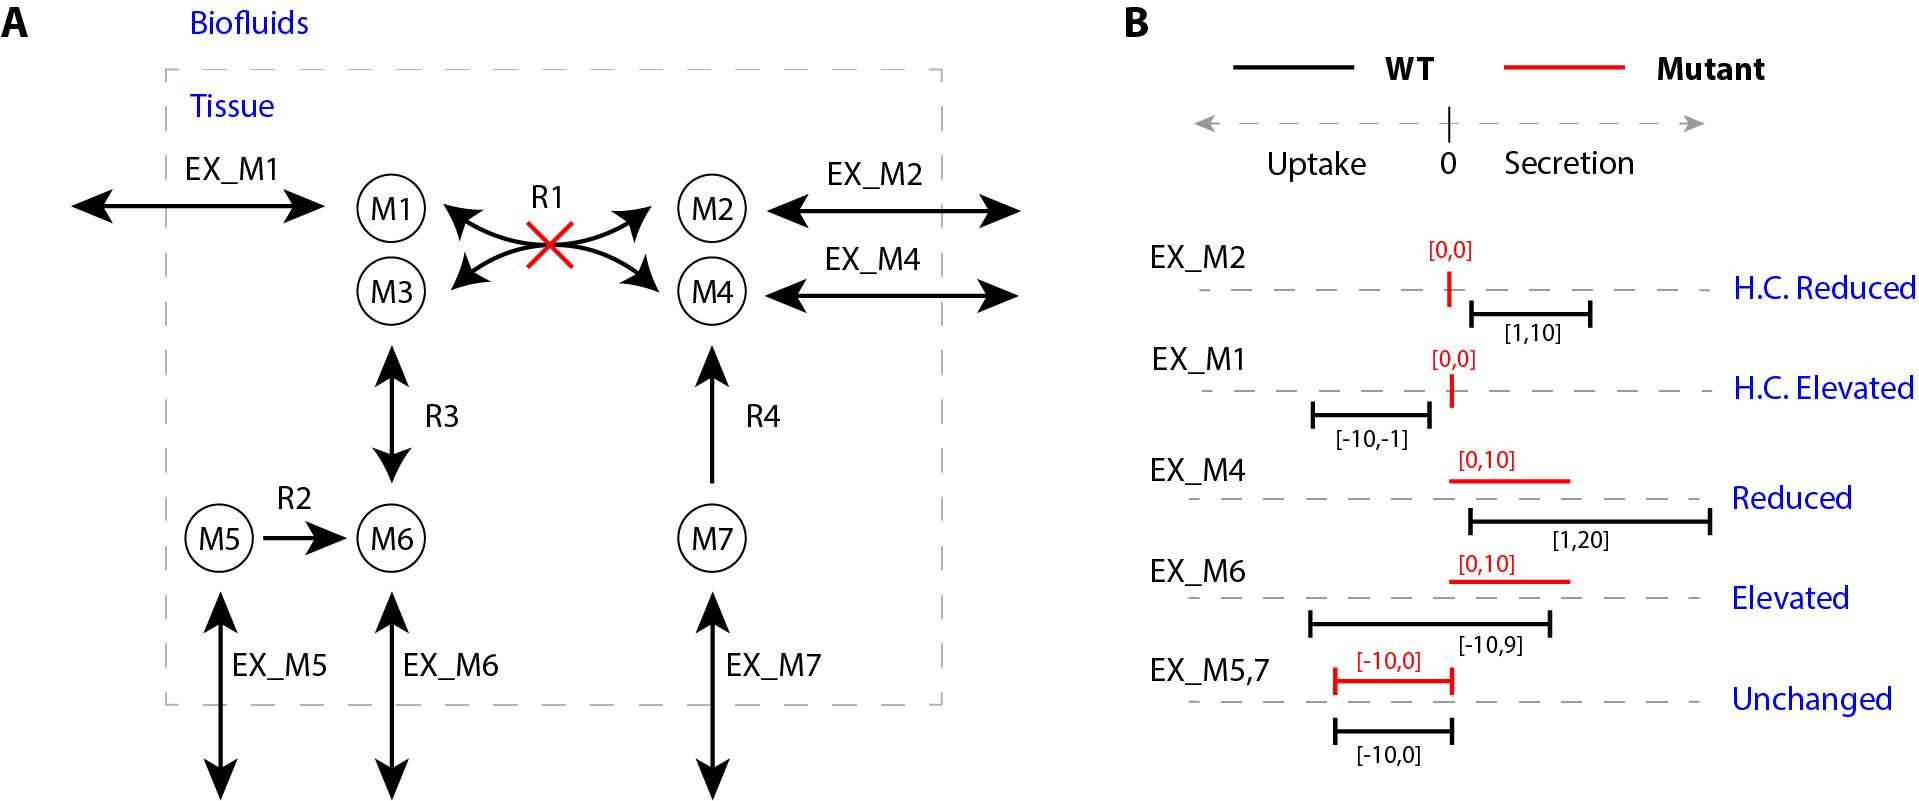
\includegraphics{Figures/Reproduction_Shlomi_fig_1}
\caption{(A) A metabolic network used to illustrate the predictions of
biomarkers of IEMs as originally considered in the work by Shlomi et al.
for their prediction of biomarkers of IEMs. All metabolites but M3 have
an exchange reaction allowing for uptake or secretion of the
metabolites. M2 synthesis is fully dependent on uptake of M1 and M5 or
M6. The IEM considered is one that leads to deletion of the enzyme
converting M1 plus M3 to M2 plus M4. (B) Visual illustration of the
predicted exchange intervals for each of the metabolites with an
exchange reaction. The wild-type (WT) interval is indicated in black,
the mutant interval in red. Each interval is associated with a numeric
interval predicted by the biomarker prediction algorithm and with a
qualitative prediction for the level of the metabolite in the biofluids
(see methods). H.C. is an abbreviation for a highly confident biomarker,
see main text.}\label{fig:Shlomi2009_figure_1}
\end{figure}

The original publication's Figure 1, panel A and B, exemplified the
biomarker prediction method for an illustrative network. It is
reproduced here as Figure ~\ref{fig:Shlomi2009_figure_1}. The simple
nature of the example serves to explain the reasoning behind the method
and also helped us validate our implementation of the method. This
repository provides an SBML file of the network, the Jupyter notebook
that generates it and a Jupyter notebook reproducing the biomarker
prediction. The image itself was produced using Adobe Illustrator.

The network in Figure ~\ref{fig:Shlomi2009_figure_1}A consists of seven
metabolites, \(6\) of which (i.e.~all except M3) have exchange
reactions. We consider a hypothetical deletion of the enzyme catalyzing
the conversion of M1 into M2 coupled to the conversion of M3 into M4.
Shlomi et al. graphically provide the biomarker prediction for this
network in their Figure 1A. Here, we do so graphically and numerically
in Figure ~\ref{fig:Shlomi2009_figure_1}B and this paper is accompanied
by a Jupyter notebook reproducing the biomarker prediction. In our
analysis, all exchange reactions were given inward bounds of \(-10\) and
outward bounds of \(+1000\) so that the internal reaction bounds (of
\(\pm 1000\)) are never reached. Figure ~\ref{fig:Shlomi2009_figure_1}B
shows that all exchangeable metabolites except M5 and M7 are predicted
to be robust biomarkers.

The exchange interval we found for metabolite M6 shows that in the
wild-type case, M6 can be either taken up from biofluids or secreted.
The upper bound is lower in absolute value than the lower bound because
in the wild type, at least \(1\) unit of flux is needed to provide M3 as
substrate for the enzyme under investigation since the enzyme convert M1
and M3 to M2 and M4 is required to have a minimal flux of \(1\) unit. In
the disease case, M6 (synthesized through M5) can only be secreted to
biofluids. These results are in full agreement with the original
publication.

\subsection{\texorpdfstring{Reproduction of Figure 2 in
\autocite{Shlomi2009}}{Reproduction of Figure 2 in {[}@Shlomi2009{]}}}\label{reproduction-of-figure-2-in-shlomi2009}

Shlomi et al. applied their method to the reconstructed human metabolic
map, examining a set of \(17\) IEMs affecting amino-acid metabolism.
Figure 2 in their publication compares predicted biomarkers with known
biomarkers from the OMIM database \autocite{McKusick2007}. We reproduced
the analysis for each IEM listed in Table ~\ref{tbl:amino_acid_iems} and
ultimately found full agreement between what was reported by Shlomi et
al. and the results of our implementation.

It is worthwhile to note, with an eye on the sensitivity of this
approach to the various settings, that we needed to set the medium
composition very specifically. Shlomi et al. did not report on their
chosen medium in their publication but we were able to reproduce their
results by setting all inward flux bounds to \(-10\) and all outward
flux bounds to \(1000\).

We made use of the Excel file included as supplementary information in
\autocite{Shlomi2009} and included it in this repository as well. The
genes and reactions linked to a given IEM are detailed in this Excel
file. We attempted to extract the genes for each IEM and using the Recon
1 map, deduced the coupled reactions, but found out that this yielded
predictions different from the ones presented by Shlomi et al. However,
the reactions listed in the Excel file are not necessarily the same
reactions that are linked in Recon 1 to the genes linked to the IEMs.
Assuming the reconstruction of the metabolic network to be accurate,
this raises some doubts as to the correctness of the results obtained by
Shlomi et al. for those IEMs where the listed reactions did not agree
with the reconstructed map.

Additionally, we needed to manually add the information for
S-Adenosylhomocysteine hydrolase and Methionine adenosyltransferase
deficiency, since they were missing from the Excel file and to reduce
the tetrahydrobiopterin deficiency gene list to only consider QDPR
(quinoid dihydropteridine reductase). Lastly, Histidinemia was in the
Excel file associated to the reaction HISD whereas this should have
referred to HISDr to match the reaction identifier in Recon 1. After
these changes, we recovered the results as originally presented and as
summarized here in Table ~\ref{tbl:amino_acid_iems}.

\hypertarget{tbl:amino_acid_iems}{}
\begin{longtable}[]{@{}llll@{}}
\caption{\label{tbl:amino_acid_iems}We used our implementation to
reproduce the biomarkers for the list of inborn errors of metabolism
shown in Figure 2 in \autocite{Shlomi2009}. Using the supplementary
Excel table of \autocite{Shlomi2009} linking IEMs to causative genes and
affected reactions, we filtered out those that are listed here. The only
considered biomarkers are the \(20\) proteinogenic amino acids. We
report all biomarkers the change of which exceeds the 10\% threshold and
categorize them by their qualitative prediction: elevated or reduced
serum levels. }\tabularnewline
\toprule
IEM & Affected reactions & Elevated & Reduced\tabularnewline
\midrule
\endfirsthead
\toprule
IEM & Affected reactions & Elevated & Reduced\tabularnewline
\midrule
\endhead
S-Adenosylhomocysteine & SEAHCYSHYD, AHCi & L-Methionine &
L-Cysteine\tabularnewline
hydrolase & & &\tabularnewline
Alkaptonuria & HGNTOR & L-Tyrosine &\tabularnewline
Argininemia & ARGN & &\tabularnewline
Cystinuria & CYSTSERex, & &\tabularnewline
& SERLYSNaex & &\tabularnewline
Lysinuric protein & SERLYSNaex & &\tabularnewline
intolerance & & &\tabularnewline
Glutamate formimino- & FTCD, GluForTx & L-Histidine &\tabularnewline
transferase deficiency & & &\tabularnewline
Histidinemia & HISDr & L-Histidine &\tabularnewline
Homocystinuria & CYSTS, MTHFR3, & L-Methionine &
L-Cysteine\tabularnewline
& METS & &\tabularnewline
Hyperprolinemia type I & PRO1xm, PROD2m & &\tabularnewline
Maple syrup & OIVD1m, & L-Valine, &\tabularnewline
urine disease & OIVD2m, & L-Isoleucine &\tabularnewline
& OIVD3m & L-Leucine, &\tabularnewline
Methionine adenosyl- & SELMETAT, METAT & L-Methionine &
L-Cysteine\tabularnewline
transferase deficiency & & &\tabularnewline
methylmalonic acidemia & CBLATm, CBL2tm, & L-Isoleucine &\tabularnewline
& MMMm & &\tabularnewline
Phenylketonuria & PHETHPTOX2 & L-Phenylalanine &
L-Tyrosine\tabularnewline
Phenylketonuria II & DHPR & &\tabularnewline
Tyrosinemia type I & FUMAC & L-Tyrosine &\tabularnewline
Tyrosinemia type III & PPOR, 34HPPOR & L-Tyrosine &\tabularnewline
Glycine encephalopathy & GCC2am, GCC2bim, & &\tabularnewline
& GCC2cm, GCCam, & &\tabularnewline
& GCCbim, GCCcm & &\tabularnewline
\bottomrule
\end{longtable}

\subsection{\texorpdfstring{Reproduction of Figure 3
\autocite{Shlomi2009}}{Reproduction of Figure 3 {[}@Shlomi2009{]}}}\label{reproduction-of-figure-3-shlomi2009}

\begin{figure}
\centering
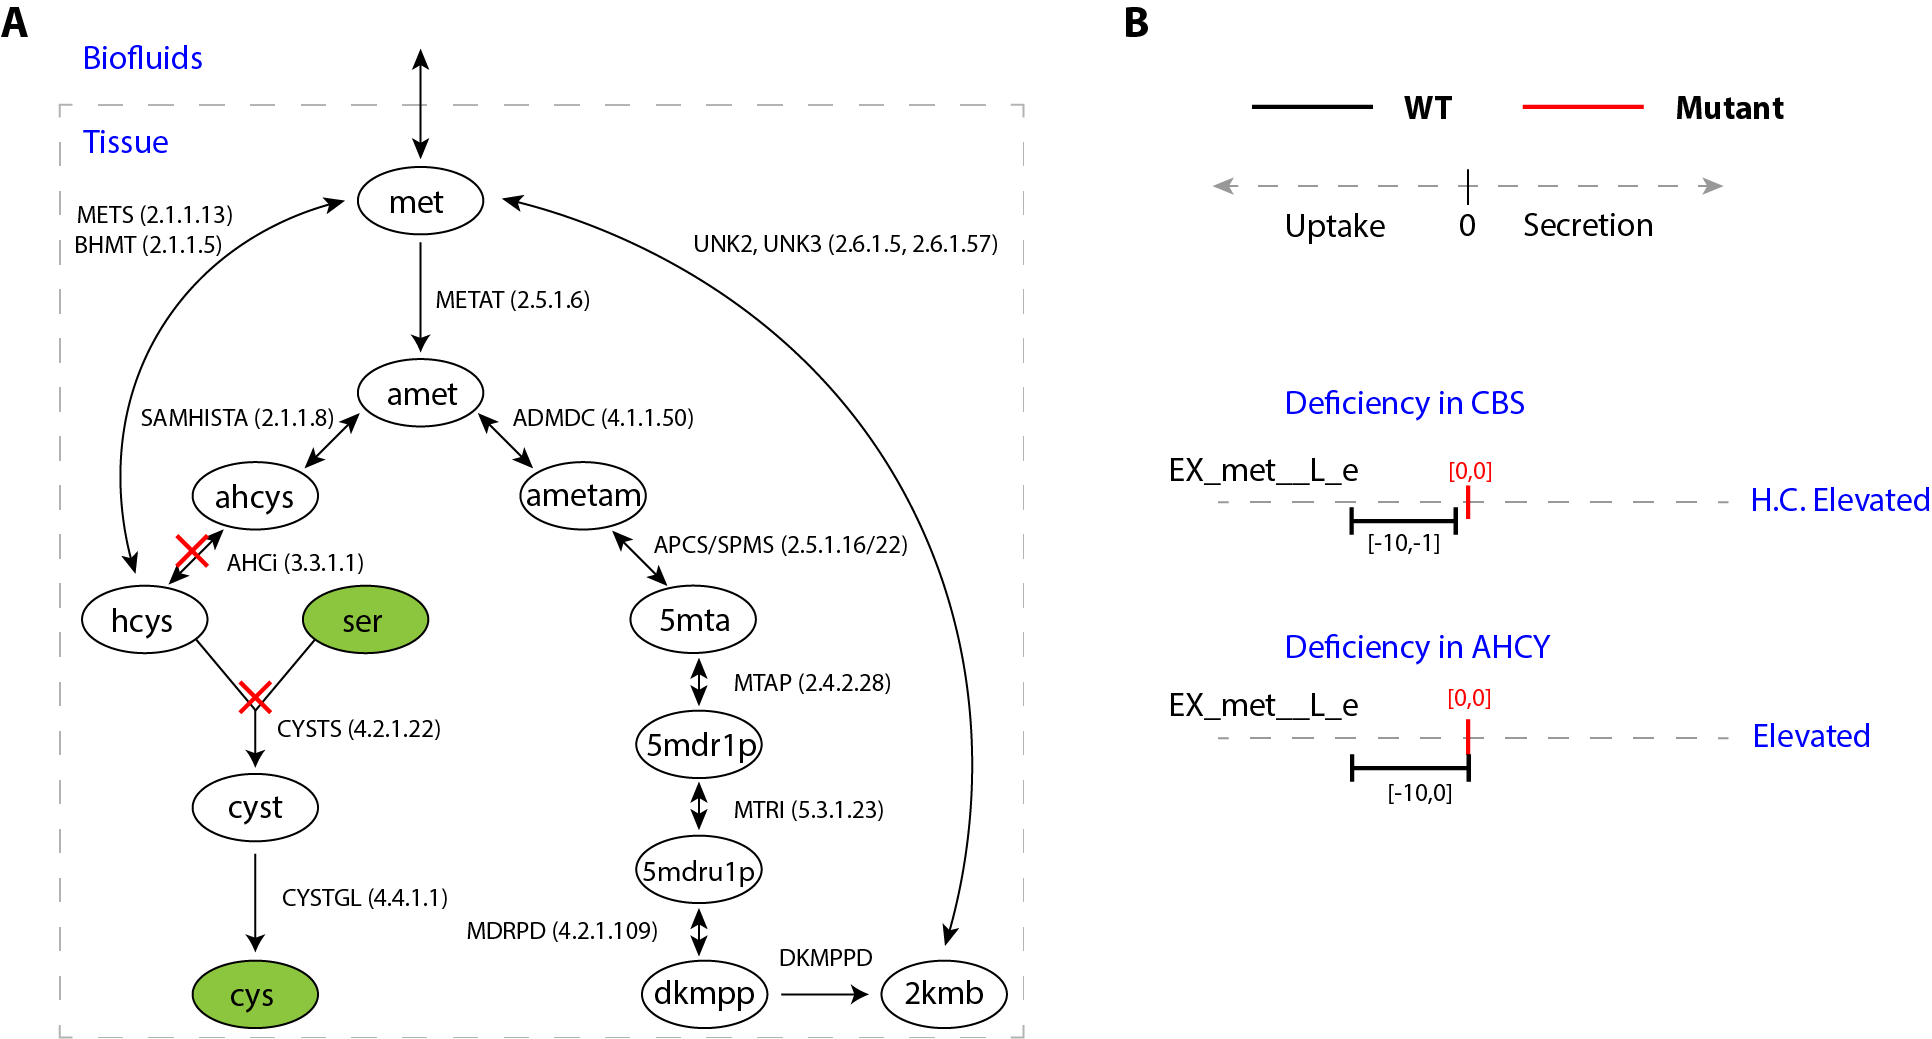
\includegraphics{Figures/Reproduction_Shlomi_fig_3}
\caption{Reproduction of Figure 3 in \autocite{Shlomi2009}. (A)
Illustration of the subnetwork of Recon 1 relevant to the effect of
homocystinuria on the metabolism and transport of methionine. Nodes
represent metabolites and edges represent reactions. For simplicity,
only abbreviations of metabolite names are given in the figure. The full
names are: L-Methionine (met), S-Adenosyl-L-methionine (amet),
S-Adenosyl-L-homocysteine (ahcys), L-Homocysteine (hcys), L-Serine
(ser), L-Cystathionine (cyst), L-Cysteine (cys),
S-Adenosylmethioninamine (ametam), 5-Methylthioadenosine (5mta),
5-Methylthio-5-deoxy-D-ribose 1-phosphate (5mdr1p),
5-Methylthio-5-deoxy-D-ribulose 1-phosphate (dmdru1p),
2,3-diketo-5-methylthio-1-phosphopentane (dkmpp),
2-keto-4-methylthiobutyrate (2kmb). Metabolites with a green background
color participate in additional reactions not shown here. Reactions are
indicated by their identifiers in Recon 1 and with a corresponding
enzyme commision number if available. We highlighted the mutations for
Homocystinuria (dysfunctional CBS) and hypermethioninemia (dysfunctional
AHCY). (B) Prediction of concentration changes of methionine in
homocystinuria and S-adenosylhomocysteine hydrolase deficiency based on
the biomarker prediction algorithm. The wild-type (WT) interval is
indicated in black, the mutant interval in red. Each interval is
associated with a numeric interval predicted by the biomarker prediction
algorithm and with a qualitative prediction for the level of the
metabolite in the biofluids (see methods). H.C. is an abbreviation for a
highly confident biomarker, see main
text.}\label{fig:Shlomi2009_figure_3}
\end{figure}

Figure 3 in the original publication entailed an in-depth look at the
effect of inborn errors in AHCY and CBS on methionine metabolism. We
reproduced this Figure as Figure ~\ref{fig:Shlomi2009_figure_3}. We used
Adobe Illustrator to redraw the network from the original publication
and based the intervals in panel B on the numerical results the
algorithm predicts. The qualitative results are already contained in
~\ref{tbl:amino_acid_iems}. The numerical results illustrated in
~\ref{fig:Shlomi2009_figure_3}B may be reproduced using the notebook
\emph{Reproduce\_figure\_2\_and\_3\_Shlomi2009.ipynb}. For clarity we
included a section in the notebook that details the results relevant to
Figure ~\ref{fig:Shlomi2009_figure_3}B.

We note that in early versions of this reproduction we were utilising a
medium that allowed influx of \(-1\) for all medium components, as
opposed to \(-10\) now. It turns out that a setting of \(-1\) does
accurately reproduce the results for Figure 2, but not for Figure 3. For
the CBS IEM the WT interval would correspond to \([-1,-1]\) and would
therefore be a point instead of a wide interval as Shlomi et al. draw
it. The reason for this stems from the forced flux \(\epsilon = 1\) in
WT. When the maximum influx of methionine is \(-1\) (as a medium
component) it is also required at a flux of \(-1\) due to the forced
active flux in the WT. When the maximum influx is increased to \(-10\)
the lower bound of the predicted interval increases to \(-10\) but the
upper bound does not because \(\epsilon\) is still equal to \(1\).

We included this simulation in the last cell of the notebook. This is
another example of the inherent sensitivity of the approach to various
settings in the algorithm.

\section{Conclusion}\label{conclusion}

The results summarized in Figures 1 (panel A and B), 2 and 3 of
\autocite{Shlomi2009} have been successfully replicated with the
software tools provided here. Overall, the reproduction process went
smoothly, since the method was applied to both an illustrative example
and to the human metabolic reconstruction, resulting in a multitude of
test cases for the implementation.

The obstacles we encountered were the lack of explicit discussion on the
set of fluxes allowed into and out of the model and a set of
discrepancies between the gene-reaction mappings listed in the
supplementary Excel file and the actual gene-reaction mappings in the
metabolic network. However, trial and error and manual curation solved
these issues.

We hope this reference implementation is useful to the community and can
serve as a starting point for further implementations of this approach
and serves as a warning of the accompanying sensitivities to various
algorithm settings we have lain out in this manuscript.

{\sffamily \small
  \printbibliography[title=References]
}
\end{document}
